\documentclass[aspectratio=169]{beamer}
\usetheme[block=fill]{metropolis}
\usepackage{tikz}
\usetikzlibrary{shapes.geometric, arrows.meta, positioning, calc}

\title{Building a Reproducible Scholarly Search Toolkit}
\subtitle{Episode 5: Query as a Research Instrument}
\author{Scholar Search Kit}
\date{}

\begin{document}

\begin{frame}[plain]
  \titlepage
\end{frame}

\begin{frame}{Episode Goal}
  \begin{alertblock}{The Goal}
    Formalize the search intent into a \texttt{Query} dataclass that acts as an auditable scientific instrument.
  \end{alertblock}
  \vspace{0.5cm}
  If a researcher says "I searched for X between 2010 and 2020", we need a programmatic way to encode, hash, and replay that exact configuration across any provider.
\end{frame}

\begin{frame}{The \texttt{Query} Dataclass}
  \begin{block}{Encoding Intent}
    We don't just pass strings around. We pass a structured \texttt{Query} object.
  \end{block}
  
  \begin{itemize}
      \item \texttt{raw\_query}: The exact boolean string (e.g., \texttt{AI AND Health}).
      \item \texttt{start\_year} \& \texttt{end\_year}: Temporal boundaries.
      \item \texttt{language}: e.g., \texttt{en} (English).
  \end{itemize}
\end{frame}

\begin{frame}{Stable Identifiers}
  \begin{center}
  \resizebox{0.65\linewidth}{!}{
  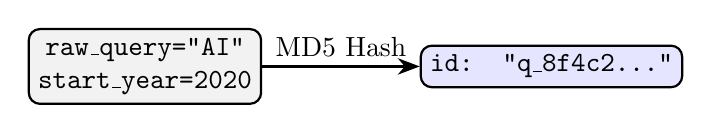
\begin{tikzpicture}[
      node distance=1.5cm and 2cm,
      box/.style={rectangle, draw, thick, rounded corners, minimum width=2.5cm, align=center, fill=black!5},
      hash/.style={rectangle, draw, thick, rounded corners, minimum width=3cm, align=center, fill=blue!10},
      arrow/.style={-{Stealth[scale=1.2]}, thick}
    ]
    
    \node[box] (query) {\texttt{raw\_query="AI"}\\\texttt{start\_year=2020}};
    \node[hash, right=of query] (id) {\texttt{id: "q\_8f4c2..."}};
    
    \draw[arrow] (query) -- node[above] {MD5 Hash} (id);
  \end{tikzpicture}
  }
  \end{center}
  \vspace{0.5cm}
  Generating a deterministic ID from the query parameters allows us to cache results and map specific documents back to the query that discovered them.
\end{frame}

\begin{frame}{Implementation: `__post_init__`}
  \begin{block}{Automatic ID Generation}
    We use Python's dataclass \texttt{\_\_post\_init\_\_} hook to automatically compute the hash ID upon instantiation.
  \end{block}
  
  \begin{itemize}
      \item This guarantees that a \texttt{Query} will \textit{never} exist without a valid, corresponding ID.
      \item Prevents developer mistakes where IDs are forgotten.
  \end{itemize}
\end{frame}

\begin{frame}{Verification}
  \begin{alertblock}{Success Criteria}
    \begin{itemize}
        \item Identical queries produce the exact same ID.
        \item Changing the \texttt{start\_year} produces a different ID.
    \end{itemize}
  \end{alertblock}
\end{frame}

\end{document}
